\hypertarget{Reverb_8h}{
\section{Reverb.h File Reference}
\label{Reverb_8h}\index{Reverb.h@{Reverb.h}}
}
{\tt \#include $<$iostream$>$}\par
{\tt \#include $<$fstream$>$}\par
{\tt \#include \char`\"{}Sound\-Sample.h\char`\"{}}\par
{\tt \#include \char`\"{}Collection.h\char`\"{}}\par
{\tt \#include \char`\"{}Track.h\char`\"{}}\par
{\tt \#include \char`\"{}Multi\-Track.h\char`\"{}}\par
{\tt \#include \char`\"{}LPComb\-Filter.h\char`\"{}}\par
{\tt \#include \char`\"{}All\-Pass\-Filter.h\char`\"{}}\par
{\tt \#include \char`\"{}Xml\-Reader.h\char`\"{}}\par


Include dependency graph for Reverb.h:\begin{figure}[H]
\begin{center}
\leavevmode
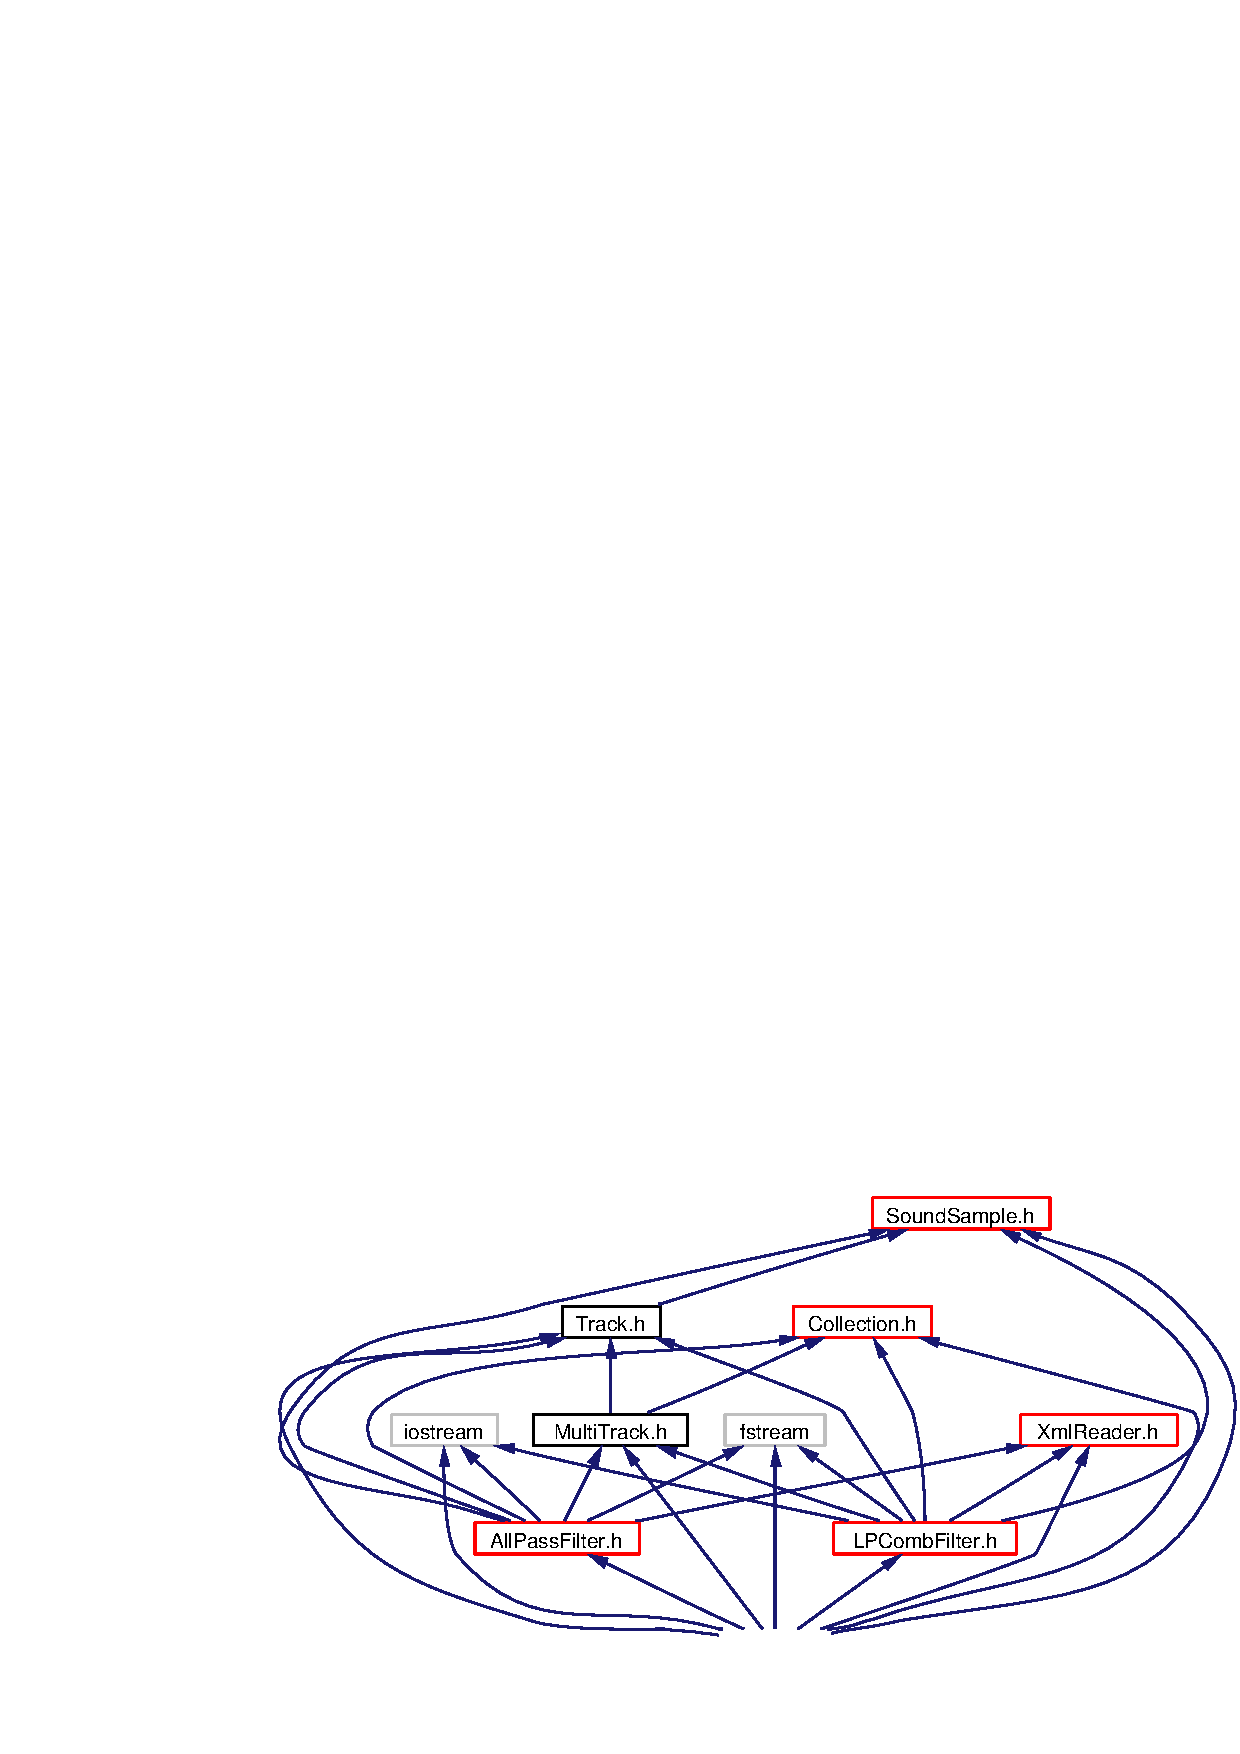
\includegraphics[width=339pt]{Reverb_8h__incl}
\end{center}
\end{figure}


This graph shows which files directly or indirectly include this file:\begin{figure}[H]
\begin{center}
\leavevmode
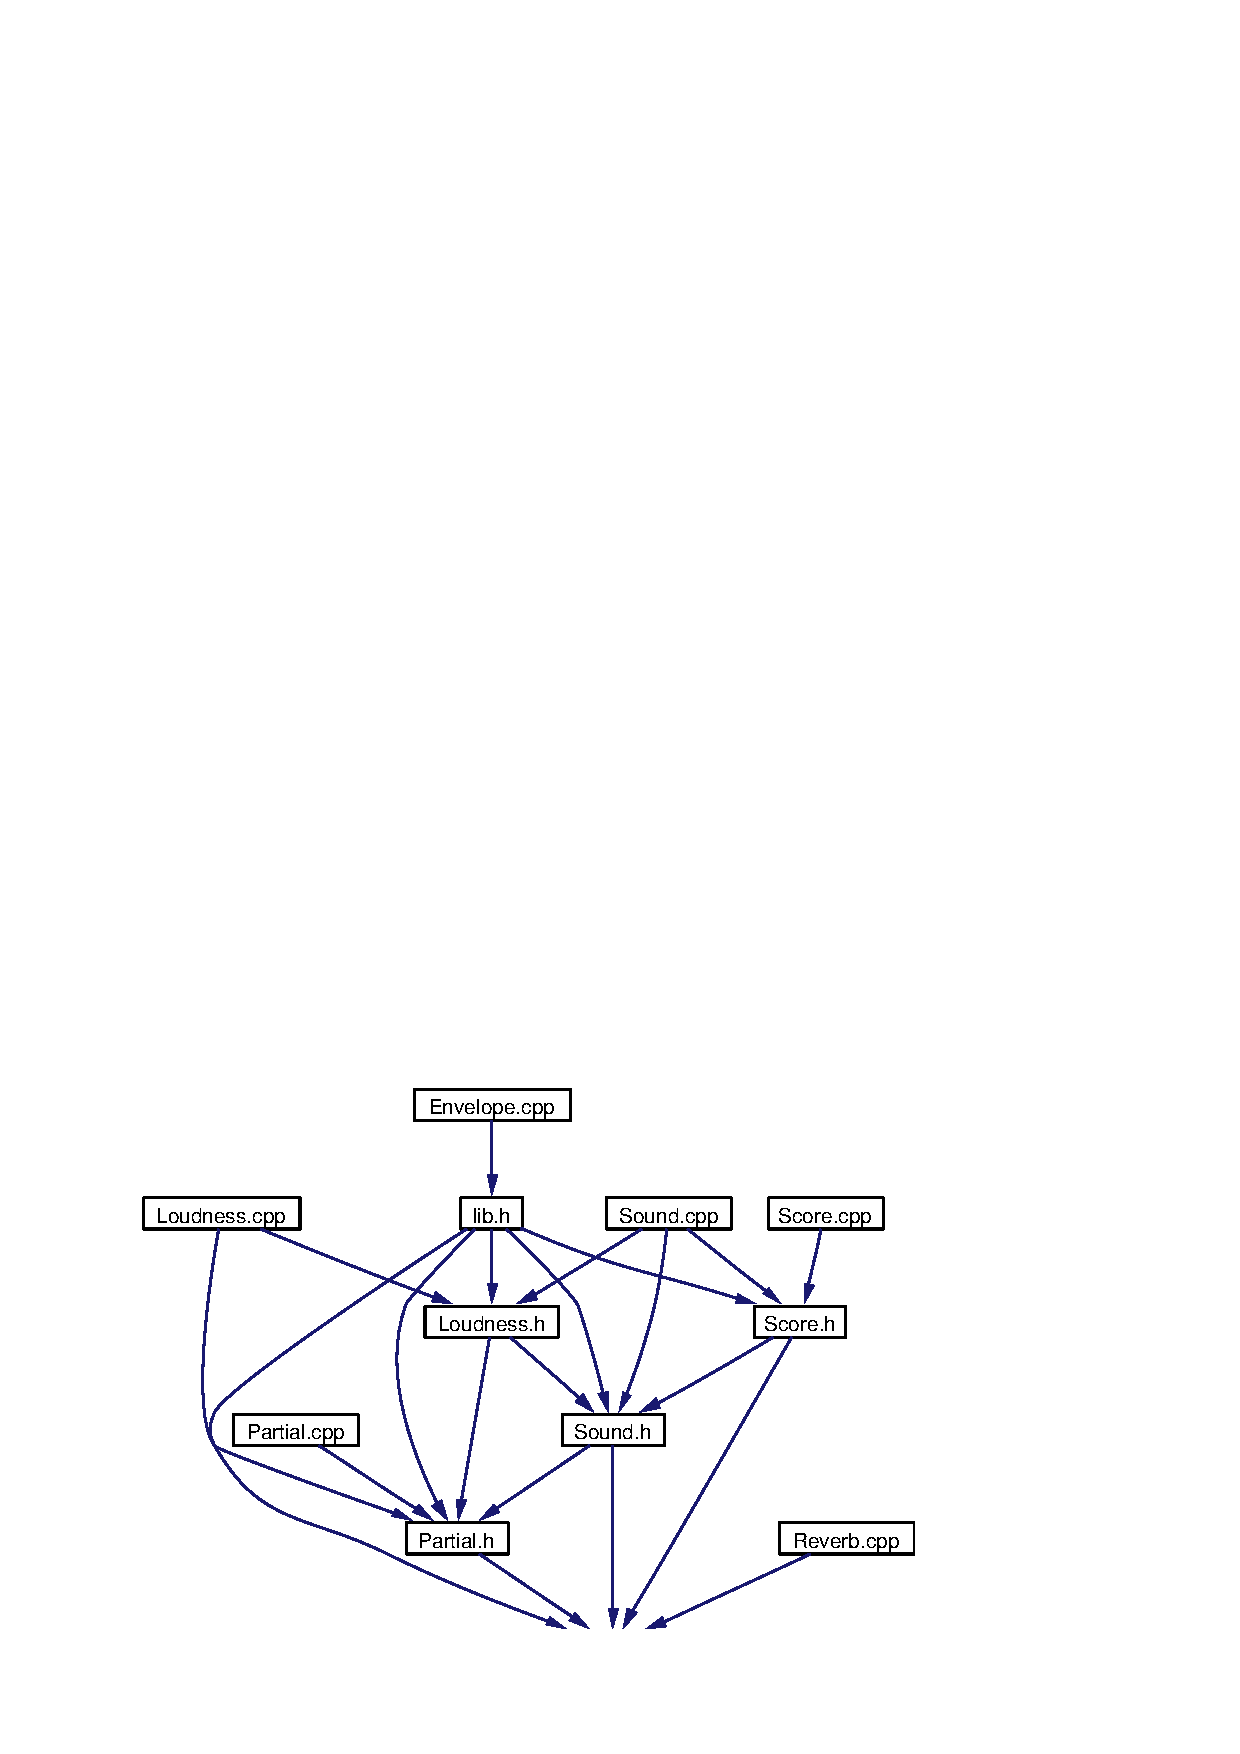
\includegraphics[width=219pt]{Reverb_8h__dep__incl}
\end{center}
\end{figure}
\subsection*{Classes}
\begin{CompactItemize}
\item 
class \hyperlink{classReverb}{Reverb}
\end{CompactItemize}
\subsection*{Defines}
\begin{CompactItemize}
\item 
\#define \hyperlink{Reverb_8h_a0}{REVERB\_\-NUM\_\-COMB\_\-FILTERS}\ 6
\end{CompactItemize}


\subsection{Define Documentation}
\hypertarget{Reverb_8h_a0}{
\index{Reverb.h@{Reverb.h}!REVERB_NUM_COMB_FILTERS@{REVERB\_\-NUM\_\-COMB\_\-FILTERS}}
\index{REVERB_NUM_COMB_FILTERS@{REVERB\_\-NUM\_\-COMB\_\-FILTERS}!Reverb.h@{Reverb.h}}
\subsubsection[REVERB\_\-NUM\_\-COMB\_\-FILTERS]{\setlength{\rightskip}{0pt plus 5cm}\#define REVERB\_\-NUM\_\-COMB\_\-FILTERS\ 6}}
\label{Reverb_8h_a0}




Definition at line 44 of file Reverb.h.

Referenced by Reverb::Constructor\-Common(), Reverb::do\_\-reverb(), Reverb::reset(), Reverb::Reverb(), Reverb::xml\_\-print(), and Reverb::$\sim$Reverb().